%Version 3.1 December 2024
% See section 11 of the User Manual for version history
%
%%%%%%%%%%%%%%%%%%%%%%%%%%%%%%%%%%%%%%%%%%%%%%%%%%%%%%%%%%%%%%%%%%%%%%
%%                                                                 %%
%% Please do not use \input{...} to include other tex files.       %%
%% Submit your LaTeX manuscript as one .tex document.              %%
%%                                                                 %%
%% All additional figures and files should be attached             %%
%% separately and not embedded in the \TeX\ document itself.       %%
%%                                                                 %%
%%%%%%%%%%%%%%%%%%%%%%%%%%%%%%%%%%%%%%%%%%%%%%%%%%%%%%%%%%%%%%%%%%%%%

%%=======================================================%%
%% to print line numbers in the margin use lineno option %%
%%=======================================================%%

%% "Numbered" switches sn-basic's citation style from author-year to the
%% numbered style the manuscript text already assumes (single \cite{key}
%% calls, no \citet-style auto-generated author names).
\documentclass[lineno,pdflatex,sn-basic,Numbered]{sn-jnl}% Basic Springer Nature Reference Style, numbered citations

%%%% Standard Packages
\usepackage{graphicx}%
\usepackage{multirow}%
\usepackage{amsmath,amssymb,amsfonts}%
\usepackage[title]{appendix}%
\usepackage{booktabs}%
%%%%

%% Manuscript notes: \NOTE, \NOTEWARN, \NOTECHECK, \NOTETODO, \NOTEQUERY.
%% Add [show] to display notes in the PDF margin, or drop the option
%% entirely for a clean submission copy (both modes degrade gracefully).
\usepackage[mark]{manuscriptnotes}

\raggedbottom

\begin{document}

\title[Selection and Relevance of Radiomic Features for Reperfusion Prediction]{Selection and Relevance of Radiomic Features for Reperfusion Prediction}

%%=============================================================%%
%% GivenName	-> \fnm{Joergen W.}
%% Particle	-> \spfx{van der} -> surname prefix
%% FamilyName	-> \sur{Ploeg}
%% Suffix	-> \sfx{IV}
%%=============================================================%%

\author[1]{\fnm{Petra} \sur{Nemcekova}}
\author[1]{\fnm{Jiri} \sur{Chmelik}}
\author[1]{\fnm{Tomas} \sur{Vicar}}
\author[2]{\fnm{Mahsa} \sur{Mojtahedi}}
\author[3]{\fnm{Manon} \sur{Kappelhof}}
\author[3]{\fnm{Jan W} \sur{Hoving}}
\author[3]{\fnm{Fabiano} \sur{Cavalcante}}
\author[9,10]{\fnm{Kilian} \sur{Treurniet}}
\author[2,3]{\fnm{Nerea} \sur{Arrarte Terreros}}
\author[2,3]{\fnm{Praneeta R} \sur{Konduri}}
\author[5]{\fnm{Aad} \spfx{van der} \sur{Lugt}}
\author[6]{\fnm{Diederik} \sur{Dippel}}
\author[8]{\fnm{Jonathan} \sur{Coutinho}}
\author[11]{\fnm{Wim} \spfx{van} \sur{Zwam}}
\author[8]{\fnm{Yvo} \sur{Roos}}
\author[3]{\fnm{Bart J} \sur{Emmer}}
\author[3]{\fnm{Charles B L M} \sur{Majoie}}
\author*[1]{\fnm{Roman} \sur{Jakubicek}}\email{jakubicek@vut.cz}
\author[2,3]{\fnm{Henk A.} \sur{Marquering}}

\affil[1]{\orgdiv{Department of Biomedical Engineering and Bioinformatics}, \orgname{Brno University of Technology}, \orgaddress{\street{Technick\'a 3082/12}, \city{Brno}, \postcode{61200}, \country{Czech Republic}}}

\affil[2]{\orgdiv{Department of Biomedical Engineering and Physics}, \orgname{Amsterdam University Medical Center}, \orgaddress{\street{Meibergdreef 9}, \city{Amsterdam}, \postcode{1105 AZ}, \country{Netherlands}}}

\affil[3]{\orgdiv{Department of Radiology and Nuclear Medicine}, \orgname{Amsterdam University Medical Center}, \orgaddress{\street{Meibergdreef 9}, \city{Amsterdam}, \postcode{1105 AZ}, \country{Netherlands}}}

\affil[5]{\orgdiv{Department of Radiology and Nuclear Medicine}, \orgname{Erasmus MC}, \orgaddress{\street{Dr.\ Molewaterplein 40}, \city{Rotterdam}, \postcode{3015 GD}, \country{Netherlands}}}

\affil[6]{\orgdiv{Department of Neurology}, \orgname{Erasmus MC UMC}, \orgaddress{\street{Dr.\ Molewaterplein 40}, \city{Rotterdam}, \postcode{3015 GD}, \country{Netherlands}}}

\affil[8]{\orgdiv{Department of Neurology}, \orgname{Amsterdam UMC}, \orgaddress{\street{Meibergdreef 9}, \city{Amsterdam}, \postcode{1105 AZ}, \country{Netherlands}}}

\affil[9]{\orgdiv{Research Bureau of Radiology and Nuclear Medicine}, \orgname{Amsterdam UMC}, \orgaddress{\street{Van der Boechorststraat 6a}, \city{Amsterdam}, \postcode{1105 AZ}, \country{Netherlands}}}

\affil[10]{\orgdiv{Department of Radiology}, \orgname{The Hague Medical Center}, \orgaddress{\street{Lijnbaan 32}, \city{The Hague}, \postcode{2262 BA}, \country{Netherlands}}}

%%% Original elsarticle source labelled this author's affiliation "DRNMM",
%%% but only defined an affiliation block labelled "CARIM" -- an undefined
%%% cross-reference that would not have compiled. Mapped here to CARIM
%%% (Maastricht UMC), the one affiliation block left otherwise unused, and
%%% consistent with this author's known institution; verify before submission.
\affil[11]{\orgdiv{Department of Radiology and Nuclear Medicine, Cardiovascular Research Institute Maastricht (CARIM)}, \orgname{Maastricht UMC}, \orgaddress{\street{UNS 50, Universiteitssingel 50}, \city{Maastricht}, \postcode{6229 HX}, \country{Netherlands}}}

%%==================================%%
%% Unstructured abstract            %%
%%==================================%%

\abstract{\NOTETODO{Draft the unstructured abstract here ($\le$200 words, no citations, no equations, no subheadings). The elsarticle draft only had the four structural labels below filled with planning notes, not actual sentences -- merge them into flowing prose once the Results/Discussion sections are finalized: Background and Objectives (why eTICI$\geq$2B prediction is clinically relevant; the gap left by van~Voorst et al., 2023, who tested one selector/classifier combination); Methods (scope of the factorial design: feature-set granularity $\times$ selection method $\times$ classifier, cross-validation plus external validation, permutation test); Results (key AUC values and their significance against the permutation baseline); Conclusions (whether the choice of feature-selection method changes the clinical conclusion).}}

\keywords{brain stroke, thrombus, radiomics, CT, feature selection}

%%% The elsarticle draft also carried an Elsevier-specific "Research
%%% highlights" list (3-5 bullets, max 85 characters each), which sn-jnl has
%%% no equivalent environment for. Kept here for reference in case another
%%% Elsevier-style submission needs it later:
%%%   - Predictive Trained models
%%%   - Trained models freely available and repository
%%%   - Explore the influence of the method and dataset to prediction accuracy?
%%%   - Explore the influence of segmentation size to prediction accuracy?
%%% It also had an (empty) \begin{graphicalabstract} placeholder, likewise
%%% dropped here for the same reason.

\maketitle

\section{Introduction}\label{sec1}

% - Klinický kontext: EVT pri veľkocievnom uzávere, eTICI škála ako outcome, prečo je predikcia úspešnosti reperfúzie klinicky užitočná (voľba stratégie/zariadenia, informovanie pacienta/tímu, procedurálne plánovanie)

Acute ischemic stroke (AIS) is caused by loss of blood circulation in a specific area of the brain due to an occlusion of an intracranial artery. AIS is one of the leading causes of mortality in the world \cite{Phipps2020}. The prognosis of the patient depends, among other factors, on findings from neuroimaging, which consists of non-contrast computed tomography (NCCT) computed tomography angiography (CTA), and sometimes CT Perfusion.

Treatment options for AIS include endovascular treatment (EVT), indicated in patients with large vessel occlusion (LVO), and intravenous thrombolysis, which can be administered if patients arrive at the hospital in time \cite{Powers2020}.\NOTECHECK[However, there is currently no protocol to determine which treatment will be most beneficial for the patient, and the final decision is dependent on radiologists' experience.]{protokol je, není nástorj na odhadnutí..to vyzníva blbě} Since each patient with suspected AIS undergoes CT imaging, recent studies have explored the potential of leveraging CT-derived imaging features for treatment outcome prediction. 
To this end, extraction of appropriate image features from CT scans is crucial to study the association between image features and clinical outcome. The extent of reperfusion can be assessed by the Extended Thrombolysis In Cerebral Infarction (eTICI) score. eTICI has therefore been suggested as a suitable parameter for differentiating between successful reperfusion and non-successful reperfusion. An estimate of the likelihood of reperfusion based on pre-treatment data could aid procedural planning and help maximize the benefit of EVT for the patient.

% - State of the art zameraný na: (a) radiomika trombu vo všeobecnosti,

Radiomics \NOTECHECK[\cite{Qiu2018}]{Gillies2016 nebo Aerts2014?}, a method for the extraction of a vast amount image characteristics, has garnered attention. This approach involves the extraction of numerous image features, including first-order statistics, gray level run length matrices, neighboring gray tone difference matrices, and shape-based characteristics of the region of interest, which are imperceptible to the human eye.
Hofmeister et al. \cite{Hofmeister2020} demonstrated the efficacy of clot-based radiomic features in predicting the mechanical thrombectomy strategy for successful recanalization of patients with AIS.
Qiu et al. \cite{Qiu2018} showed the association radiomic-based features on NCCT and CTA images and the efficacy of the recanalization with intravenous alteplase. These findings underscore the potential of radiomics as a valuable tool for extracting meaningful information from medical images, contributing to improved decision-making in the treatment of stroke patients.

% (b) konkrétne van Voorst et al. 2023 — čo urobili, aké AUC dosiahli pre eTICI≥2B (~0.52–0.56, teda blízko náhode), aký feature-selection použili (ICC≥0.75 filter, RF, žiadny ďalší výber príznakov)

van Voorst et al. \cite{vanVoorst2022} identified the association of thrombus volume and texture with the number of retrieval attempts needed for successful reperfusion. However, they did not observe any additional value of thrombus radiomics for the prediction of reperfusion compared to clinical baseline variables.

% - Gap/limitácia predchádzajúcej práce: jedna pevná kombinácia feature-selection + klasifikátor; žiadne porovnanie granularity príznakov (voxel/distribution/global, whole vs. skeleton); žiadny permutačný test proti empirickému chance-baseline; žiadne overenie, či iná metóda výberu príznakov (Lasso/RFI) alebo klasifikátor (SVC) zmenia záver

Even though there are many studies that assess the association of radiomic features with clinical outcome, to the best of our knowledge, \NOTECHECK[none of them exploited the potential of information hidden in the available data and used only the mean values of the extracted features from the thrombus.]{nemyslím si že je pravda} Moreover, previous studies use radiomic feature selection based on similarity of features, Here we present an approach where radiomics features are selected using supervised approaches.

% - Research question / hypotézy — formulovať explicitne, napr.:
%   - Ovplyvňuje voľba metódy výberu príznakov a granularity feature-setu diskriminačný výkon pri predikcii eTICI≥2B?
Our study focuses on the exploration of features at different spatial scales, from global thrombus-level  to single voxel descriptors. Moreover, we investigate the influence of the segmentation size on the prediction success.

%   - Zlepší kombinovanie (ensemble/boosting) viacerých slabých modelov výkon nad rámec ktorejkoľvek jednotlivej pipeline?

% - Príspevky/novelty (mapujú sa priamo na Highlights) — systematickosť dizajnu, permutačný baseline namiesto flat 0.5, externá validácia, ensemble analýza ako „stress test" záveru

% - Slovo eTICI se v celem beznem textu neobjevi ani jednou, jen v komentarich. Ctenar tedy nevi, co vlastne predikujeme. Definovat skalu (Zaidat2013) a rict, ze cilime na 2C/3, ne na >= 2B. Duvod pro prisnejsi rez dodá LeCouffe2020 (aOR 1,34 na kazdy stupen).

% - roc je predoperacni odhad vubec k necemu. Reperfuze na prvni pokus ma lepsi funkcni vysledek nez po opakovanych pokusech (Zaidat2018), takze odhad predem informuje planovani.

% - ozptyl publikovanych vysledku: van Voorst 0,52 pro >= 2B, Xiong2023 0,850, Zhao2026 0,86, Yan2026 0,847 pro klot proti 0,719. Ruzne endpointy, ruzne ROI, ruzne selektory.

% - Nikde nestoji, proc bereme obe modality. NCCT nese podil erytrocytu (Liebeskind2011), kontrastni prirustek na CTA jde opacnym smerem (Cruts2023: fibrin 31-38 HU a prirustek 82-127 HU proti RBC 72-89 HU a prirustku 3-17 HU).

% - říct že je potřeba permutační baseline - a clanky to nedělají...motivace důležitosti tothoto

% - chybi explicitni otazky a prispevky - permutacni baseline misto plosne 0,5, externi validace, ensemble

\section{Results}\label{sec2}

\subsection{Performance across selector--classifier--feature-set combinations}
\label{sec:results:factorial}

\begin{figure}[!htb]
\centering
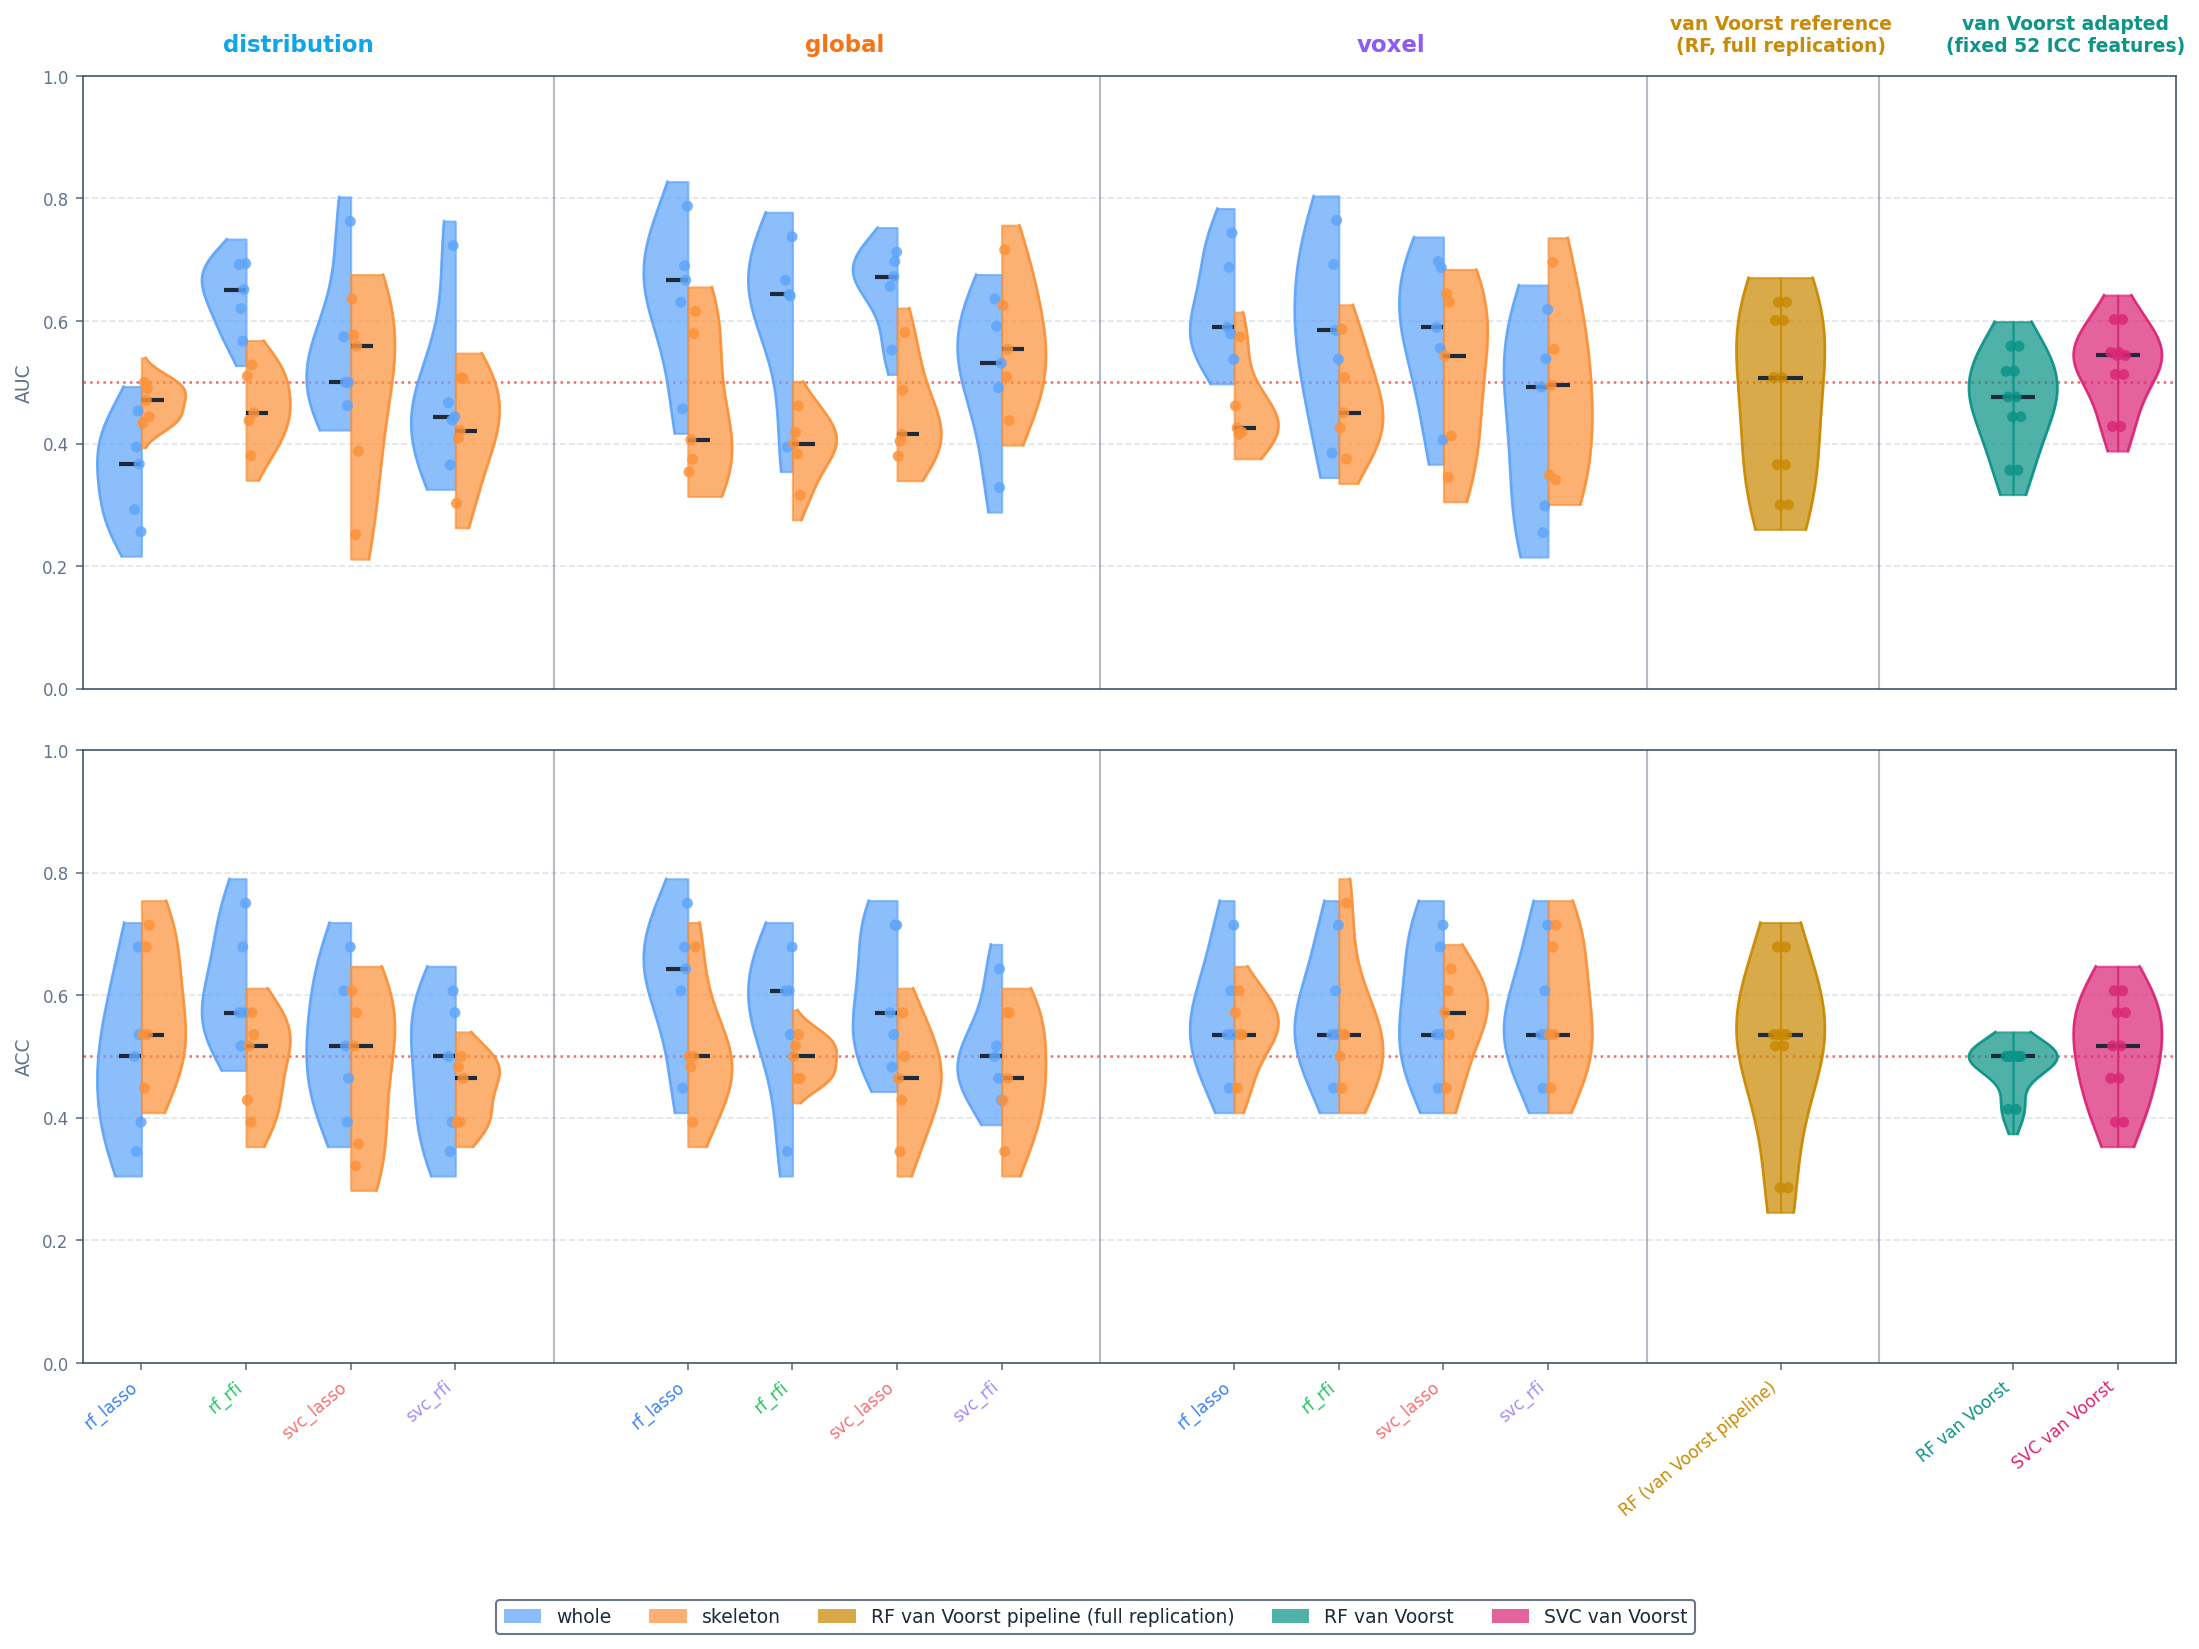
\includegraphics[width=1\textwidth]{img/05_07_auc_acc_method_fset_with_henk.png}
\caption{AUC (top) and ACC (bottom) distributions across the 24 evaluated selector--classifier--feature-set combinations. Results are grouped by feature set type: distribution-based, global-based, and voxel-based. Within each group, individual violin plots correspond to one selector--classifier combination. The left (blue) half of each violin plot represents models trained on whole-thrombus features; the right (orange) half represents models trained on features from the thrombus centerline dilated by 3~voxels. Dots represent the five individual folds and the horizontal bar represents the median. The dotted red line marks the chance level of~0.5. RF: random forest classifier; SVC: support vector classifier; RFI: random forest importance-based selector; LASSO - least absolute shrinkage and selection operator selector.}
\label{fig.AUC_ACC_distributions_all}
\end{figure}

This section show to what extent the choice of selector, classifier, feature set and region of interest alone can alter discriminative performance within a single development cohort.
Later, these results are compared with a null model and with a reference pipeline. Fig.~\ref{fig.AUC_ACC_distributions_all} shows the resulting distributions and \NOTETODO[S\ref{tab:S1-auc-acc-distributions}]{skontrolovat tabulku se statistikama do suplementu} lists the per-combination values.

Median cross-validated AUC across the 24 combinations ranged from 0.367 to 0.673, the four whole-thrombus global combinations being the highest as a group (0.632--0.673) and no centerline combination of either patient-level set exceeding 0.559.

Accuracy has to be read against the majority-class accuracy of the development cohort ($82/141 = 0.582$) and not against 0.5: only 4 of the 24 combinations exceeded it by median accuracy, and because the proportion of successful reperfusion varied between 0.448 and 0.714 across the outer folds, accuracy is meaningful only fold-wise.

Restricting the region of interest to the dilated centerline removed the discrimination present on the whole thrombus in the global-based set, where all four combinations fell from 0.632--0.673 to below chance (0.400--0.497); in the distribution-based set the effect was not consistent, the two combinations that had discriminated on the whole thrombus losing that discrimination while the two that had not changed little.

\NOTETODO[CI]{bootstrap CI pro AUC -- potreba per-pacientske skore nasich modelu na CV foldech, v datech nejsou}

\subsection{Comparison against the permutation null}
\label{sec:results:permutation}

\begin{figure}[!htb]
\centering
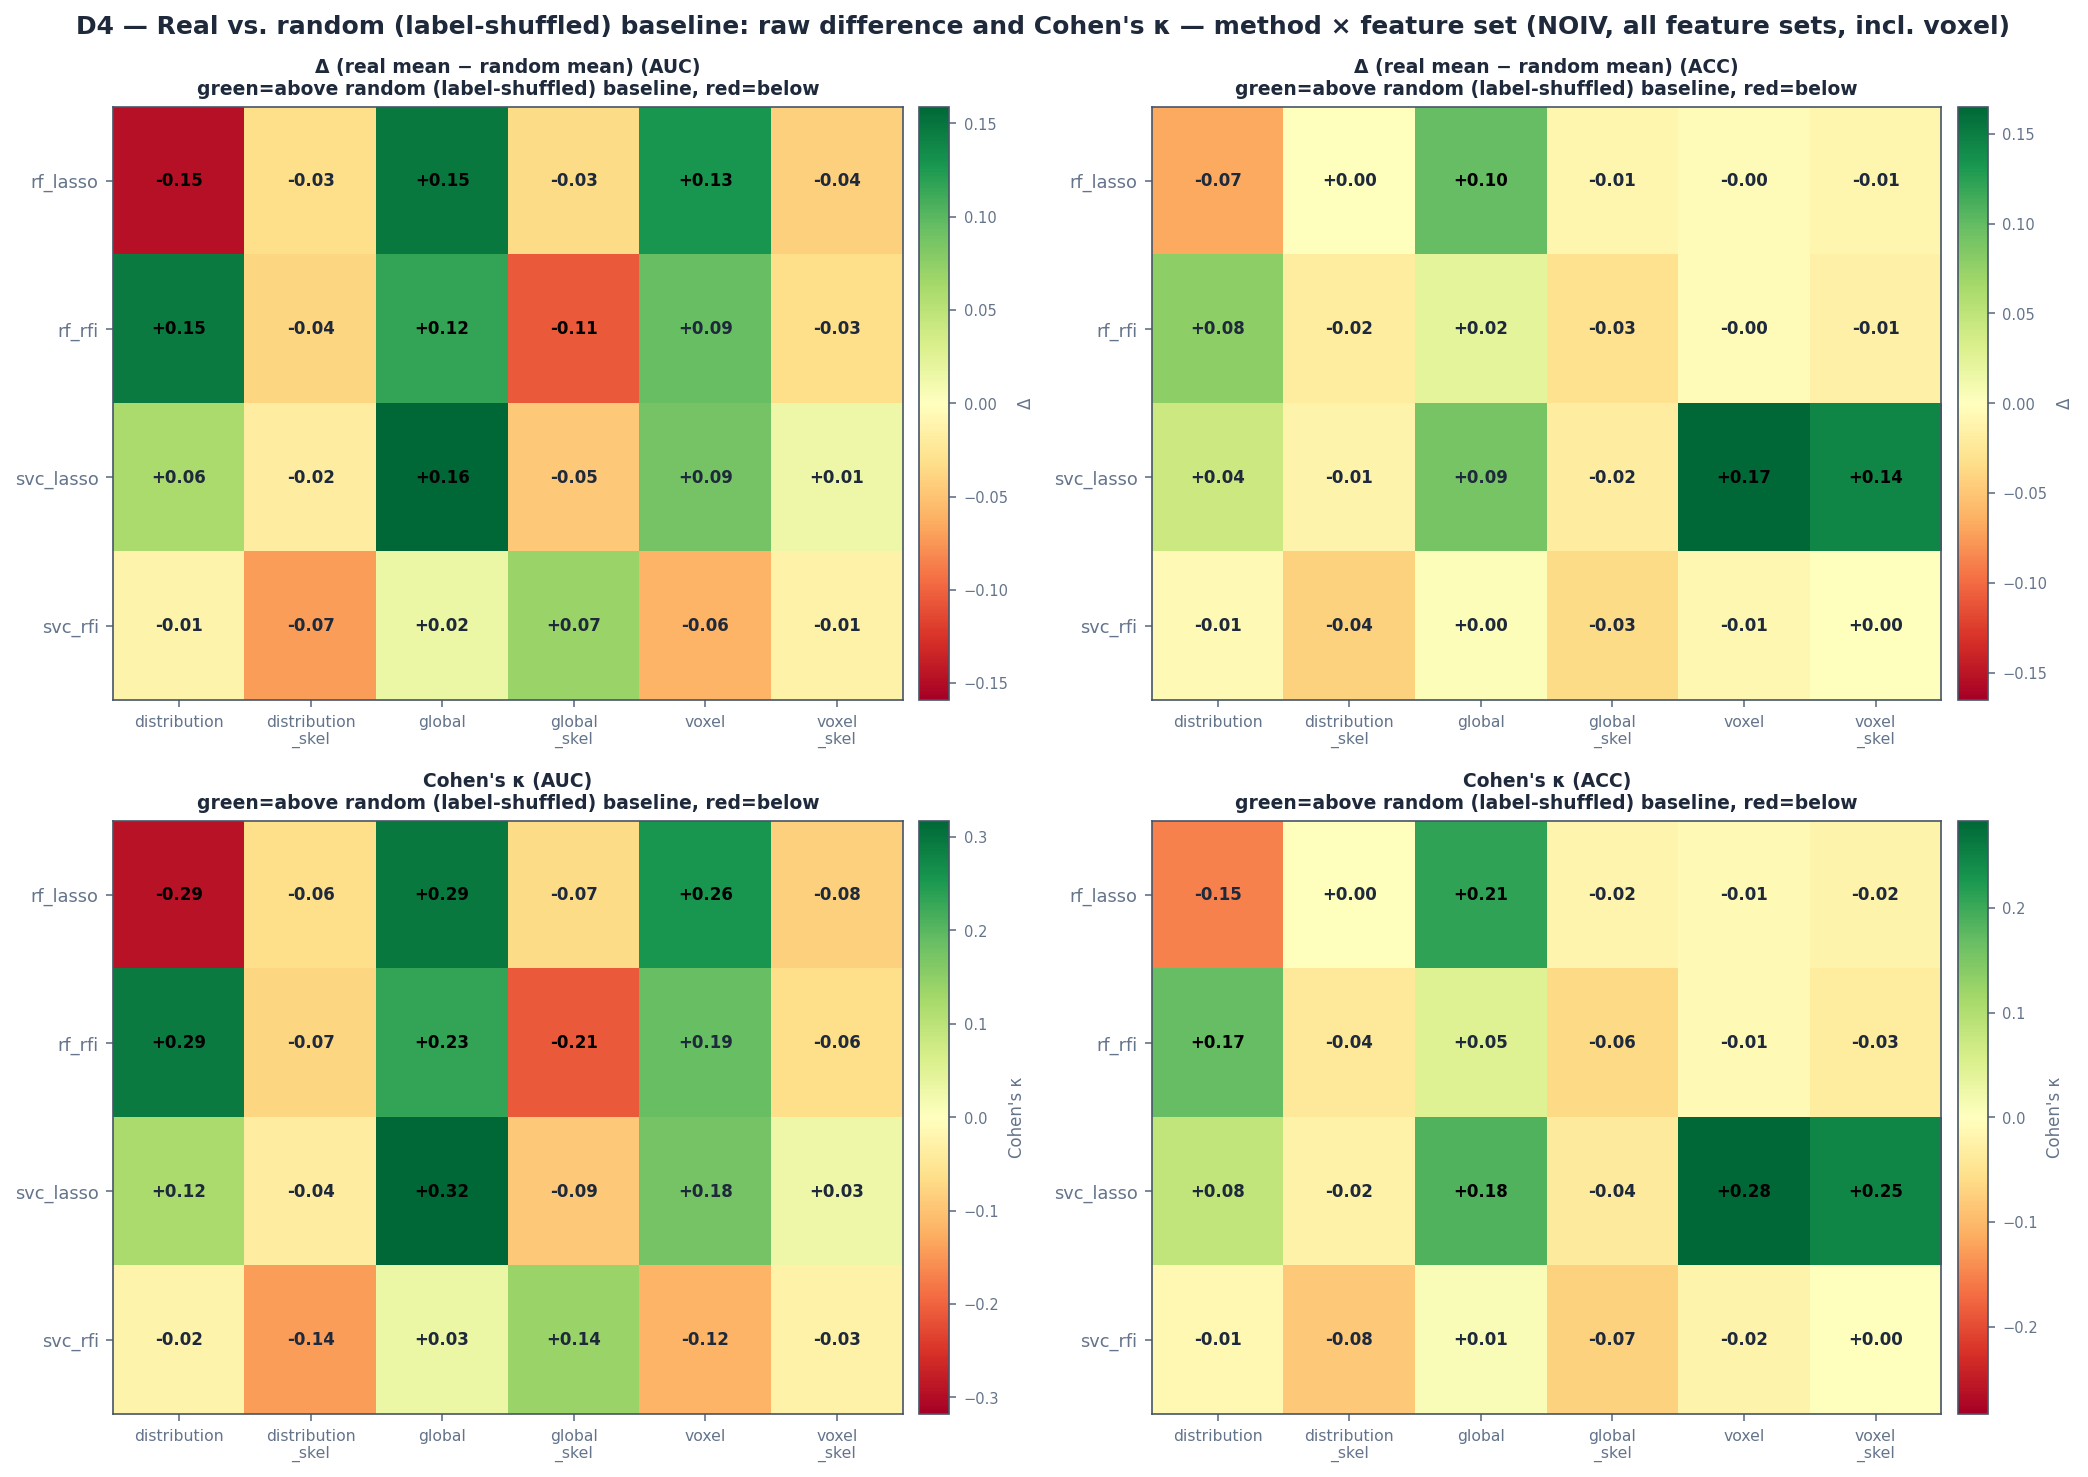
\includegraphics[width=1\textwidth]{img/D4_diff_and_kappa_heatmap_all_fsets.png}
\caption{Performance of each model compared to its randomized variant. For every selector--classifier--feature-set combination, the labels of the test set were randomly shuffled 5000~times, and the mean over these permutations is considered the performance of the random model. The top row shows the difference between the model and its randomized variant for AUC (left) and ACC (right). The bottom row shows the same comparison expressed as Cohen's~$\kappa$. Green cells represent combinations performing above their randomized variant, red cells below it. RF: random forest classifier; SVC: support vector classifier; RFI: random forest importance-based selector; LASSO - least absolute shrinkage and selection operator selector.}
\label{fig.D4_cohens_kappa_heatmap_all_fsets}
\end{figure}

This section asks whether the performance reported above exceeds what the same pipeline achieves on randomised outcome labels, because a flat chance level of 0.5 is only an assumption about where a random model would land and need not hold for every metric or every unit of analysis. Fig.~\ref{fig.D3_cohens_kappa_heatmap_all_fsets} shows each combination against its own null.

\NOTETODO[pospat princip statistiky tady počítané]{dodělat statistiku a podle toho upravit}
% The null was built separately for every combination by permuting the patient-level outcome labels 100 times within each outer test fold, holding the selected features and the fitted classifier fixed, and the test statistic was the mean AUC over the five folds; with 100 permutations the smallest attainable $p$-value is 0.0099, and because the model is not refitted the null does not absorb the optimism of feature selection and tuning.

\NOTECHECK[For AUC, 6 of the 16 patient-level combinations reached $p < 0.05$ uncorrected, all of them on the whole thrombus and with $\kappa$ between $+0.225$ and $+0.359$, three of them at the resolution floor of $p = 0.0099$.]{předběžná čísla - můžou se změnit, pak dopsat i pro ACC}

\subsection{Comparison against the reference pipeline}
\label{sec:results:reference}

\begin{figure}[!htb]
\centering
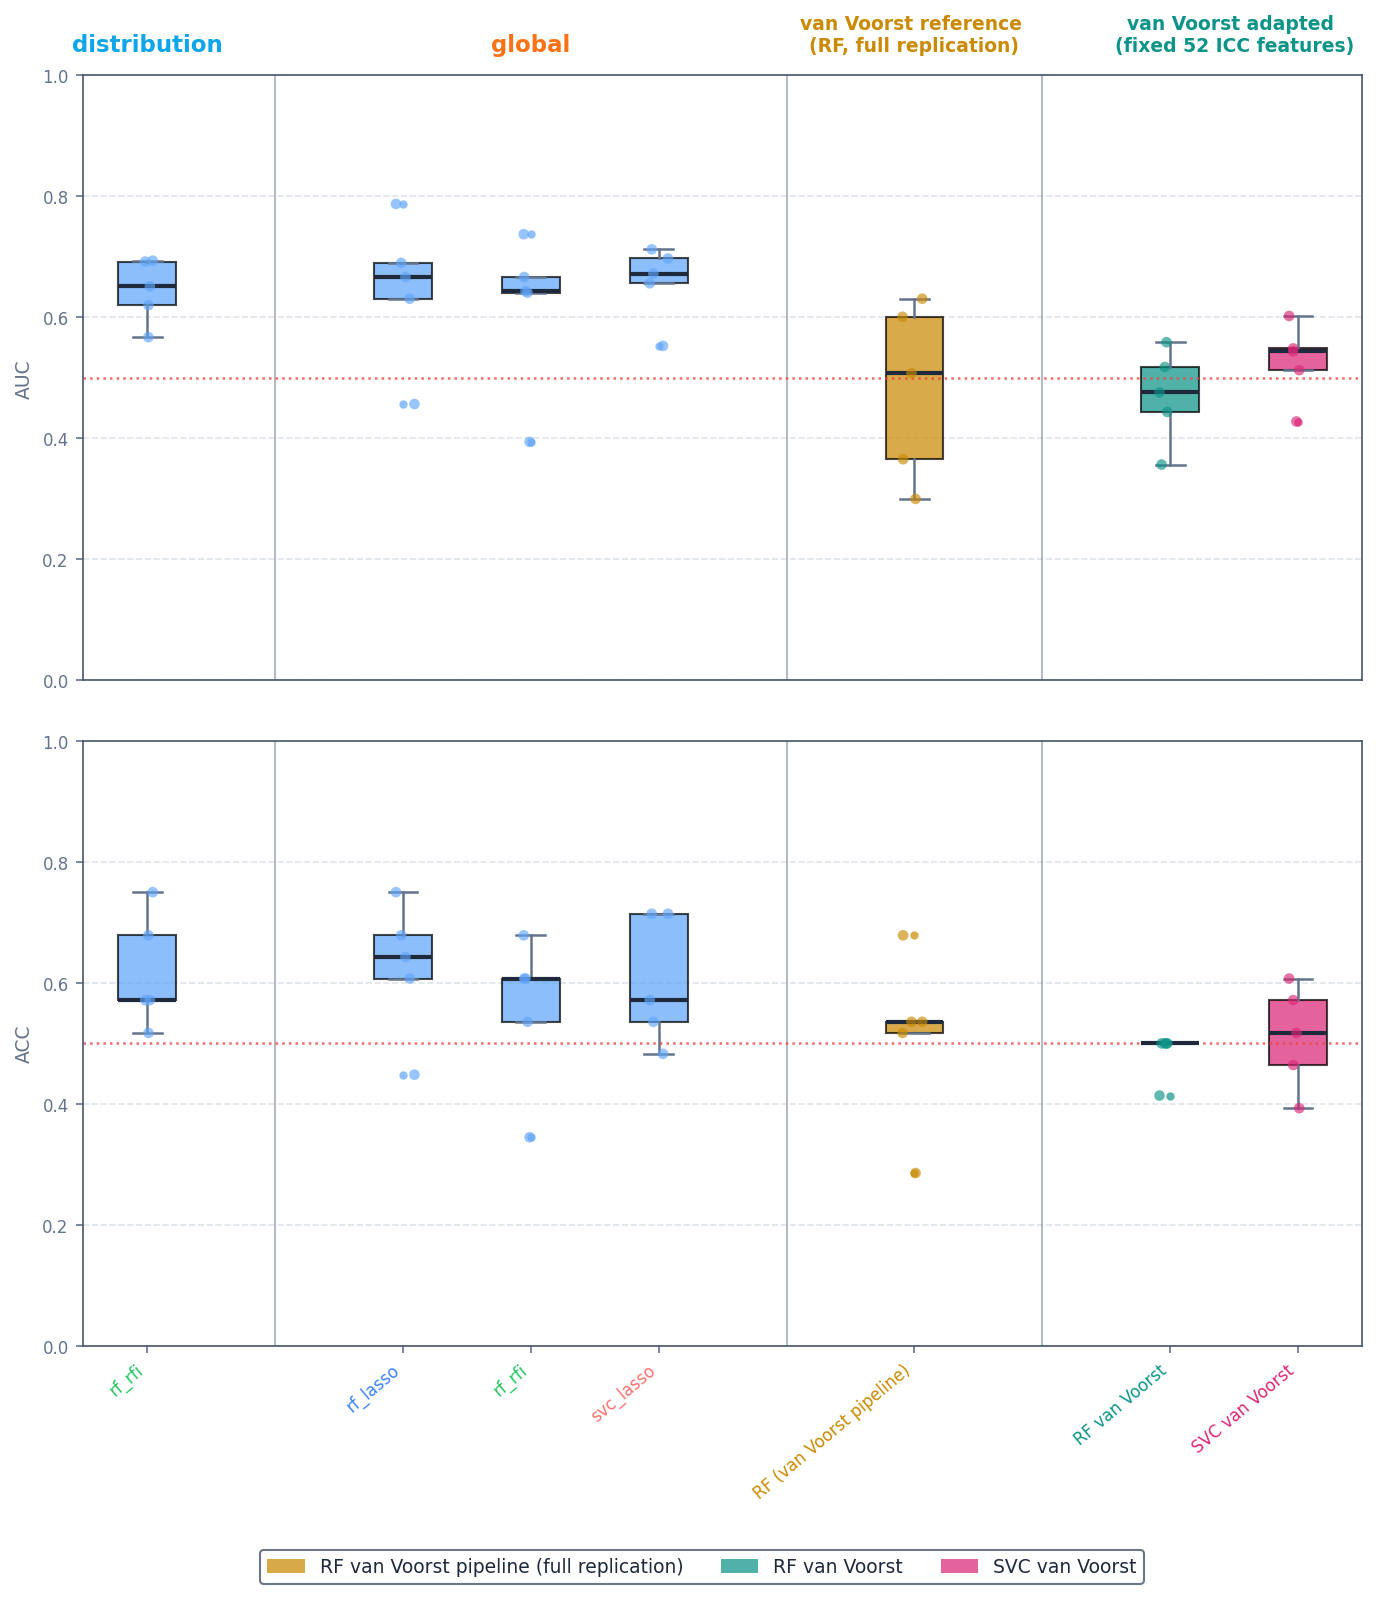
\includegraphics[width=1\textwidth]{img/auc_acc_selected_vs_henk_pipeline_boxplot}
\caption{AUC (top) and ACC (bottom) of the selected proposed combinations and of the reference pipeline of van~Voorst et al. \cite{vanVoorst2022}. Blue boxes represent the selected whole-thrombus distribution-based and global-based combinations. The yellow box represents a full replication of the reference pipeline, including its own feature selection. The green and pink boxes represent our RF and SVC classifiers trained on the fixed set of 52~ICC-filtered features reported in the reference work. Boxes show the median and the interquartile range over the five folds, and dots represent the individual folds. The dotted red line marks the chance level of~0.5. RF: random forest classifier; SVC: support vector classifier; RFI: random forest importance-based selector; LASSO - least absolute shrinkage and selection operator selector.}
\label{fig.auc_acc_selected_vs_henk_pipeline}
\end{figure}

This section asks whether the modest discrimination reported so far is a property of thrombus radiomics in this cohort or of the analysis choices made here, by recomputing a published pipeline for the same task on the same patients and the same folds and placing it next to the proposed combinations. Fig.~\ref{fig.auc_acc_selected_vs_henk_pipeline} places the two side by side and \NOTETODO[Table SXXX]{srovnani s referencni pipeline} lists the fold-wise differences.

\subsection{External validation on the MR CLEAN Registry}
\label{sec:results:external}

\begin{table}[h]
\caption{Caption}\label{tab:placeholder}%
\begin{tabular}{@{}cc@{}}
\toprule
 & \\
\midrule
 & \\
\botrule
\end{tabular}
\end{table}

This section asks whether any of the pipelines retains its discriminative performance once it is moved to a cohort it was not developed on, which is the question that cross-validation within a single curated dataset cannot answer. \NOTETODO[Table SXXX]{externi validace CV median vs. Registry vcetne delta AUC -- table4_external_validation, nahradit prazdnou tab:placeholder} lists the cross-validated and the external values side by side.

\NOTETODO[statistika do tabulky]{tabulka porovnani naseho nejlepsiho modelu vs. jeho permutacni varianty vcetne statistickeho testu + porovnat Henkuv s nasim na stejnem setu z Registry + statisticky test - zkusit pouzit bagging?}

\section{Discussion}\label{sec3}

\NOTEWARN[Duplicate figures/labels below]{This Discussion re-plots \texttt{05\_07\_auc\_acc\_method\_fset.png} and \texttt{D4\_diff\_and\_kappa\_heatmap\_all\_fsets.png} in new \texttt{figure} environments reusing the labels \texttt{fig.AUC\_ACC\_distributions\_all} and \texttt{fig.D3\_cohens\_kappa\_heatmap\_all\_fsets} already defined in Section~\ref{sec2}. Left as-is per author decision (2026-09-14) rather than resolved during this template port -- this needs the duplicate figures removed (replaced with \texttt{Fig.~\ref{fig.AUC\_ACC\_distributions\_all}}-style cross-references to the Results copies) before this document will compile without duplicate-label warnings and doubled figures.}

The prediction accuracies (ACC) and areas under the curve (AUC) were evaluated for all methods, feature sets, and regions of interest to investigate the dependence of model performance on dataset type, area size, fold, and method used. All results are provided in supplementary file~\textit{B}.

% \begin{figure}[!htb]
% \centering
% 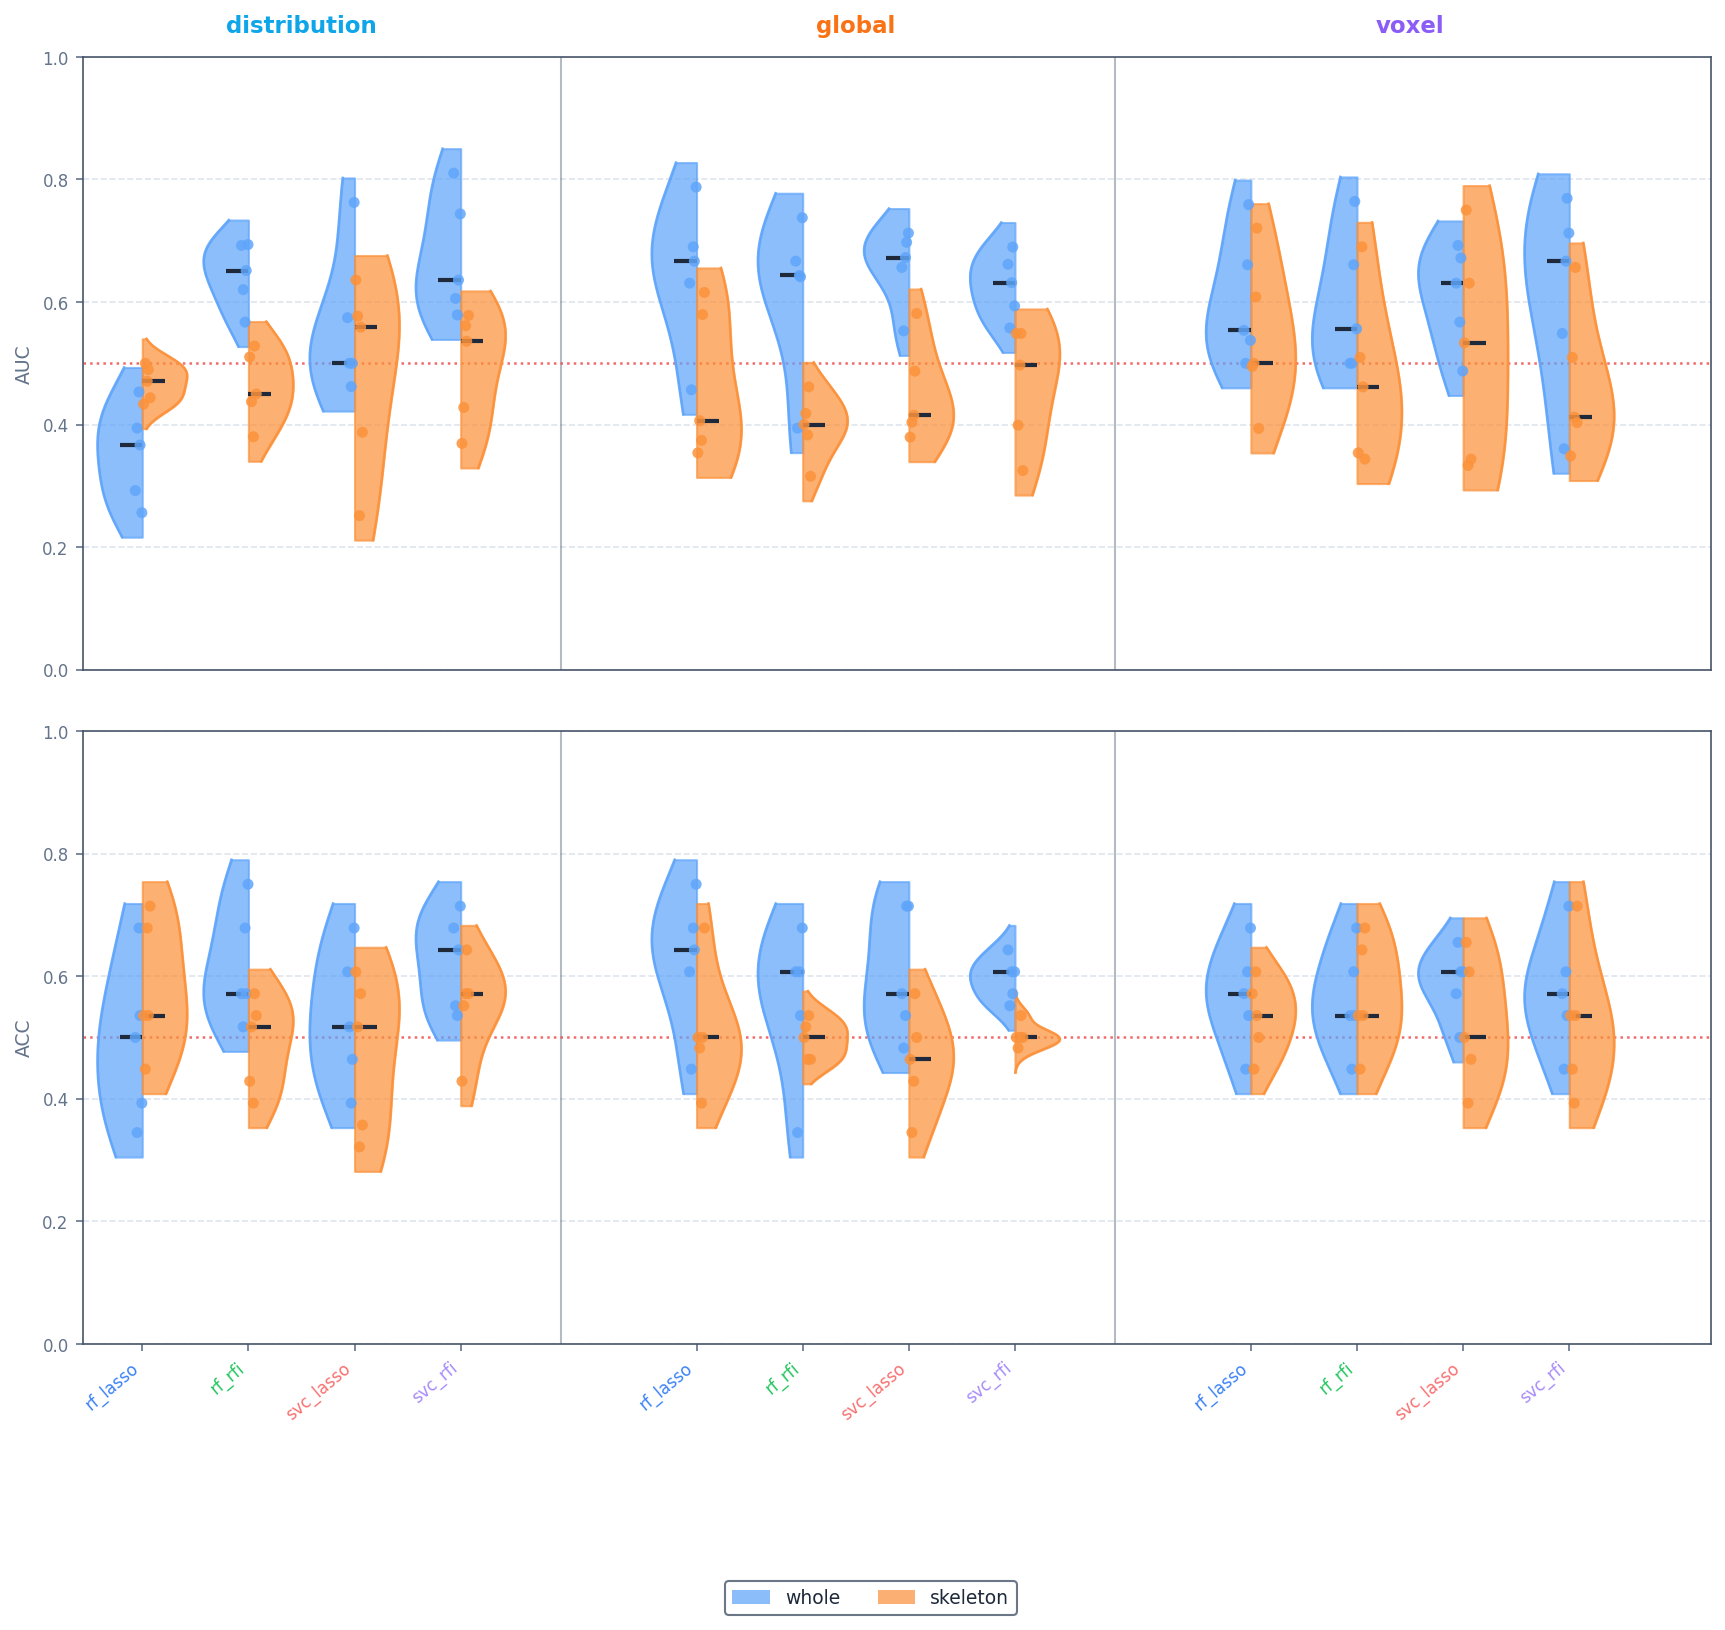
\includegraphics[width=1\textwidth]{doc/05_07_auc_acc_method_fset_corrected.png}
% \caption{AUC (top) and ACC (bottom) distributions across all evaluated classifiers and feature sets. Results are grouped by feature set type: distribution-based, global-based, and voxel-based. Within each group, individual violin plots correspond to one classifier. The left half of each violin plot represents models trained on whole-thrombus features; the right half represents models trained on thrombus core features. RF: random forest classifier; SVC: support vector classifier; RFI: random forest importance-based selector; LASSO - least absolute shrinkage and selection operator selector.}\label{fig.AUC_ACC_distributions_all2}
% \end{figure}

As visible in Fig.~\ref{fig.AUC_ACC_distributions_all}, the meaningful performance of the models decreased when only the core voxels of the thrombus were selected compared to the results achieved using the information from the whole clot. Accordingly, even though the precision of the voxel based models was high, the voxel based dataset appeared to contain insufficient information to distinguish between SRP/nSRP and led to model underfitting with the prediction of the same label regardless of the method used. These results confirm the expected findings, that the information provided by a single voxel is insufficient to establish the clinical outcome. Nevertheless, this dataset was crucial for the creation of the global and distribution based datasets.

The investigation, whether the models performance is higher than  Based on the Fig.~\ref{fig.D4_cohens_kappa_heatmap_all_fsets} of the Cohen's~$\kappa$ comparing the performance of the model to its randomized variant. The performance of the random model variant was obtained by randomly shuffling labels 100 times to the testing dataset. The mean accuracy achieved on the dataset with not true labels is considered as the accuracy of the random model with the same architecture and parameters as the predictive one.

Due to the findings stated, further analysis will focus on the distribution and global based whole thrombus datasets. Results achieved using information only from the thrombus centerline and voxel-based dataset may be viewed in the supplementary material.

The median AUC of the models using the global-based feature set was above 63\%, and the median ACC was higher than~57\%. These results substantially exceed the performance reported by~\cite{vanVoorst2022}, who achieved an AUC of~52\% for SRP prediction using only mean global thrombus radiomic features.

In the case of the models using the distribution-based information, the median AUC of the LASSO-RF model achieved only~37\% and median ACC was~50\%. As visible in Fig.~\ref{fig.spline_combined_dist_global}, models using this method utilized only one feature for classifier training, when using the distribution-based dataset. Based on the results, the model was not able to fit appropriately during the entire optimization process, which resulted in a set of zero weighted coefficients for all provided features. Since all features were determined to be equally unimportant due to their low relationship with the SRP/nSRP, only the probability density in the first bin of the histogram created from the NCCT thrombus scan was selected for training. However, even though the median metric values of the rest of the classifiers reach almost the same fruitfulness as a random classifier, some models reach AUC and ACC above 70\%, which suggests that the distribution based features introduce clinically relevant information.

\begin{figure}[!htb]
\centering
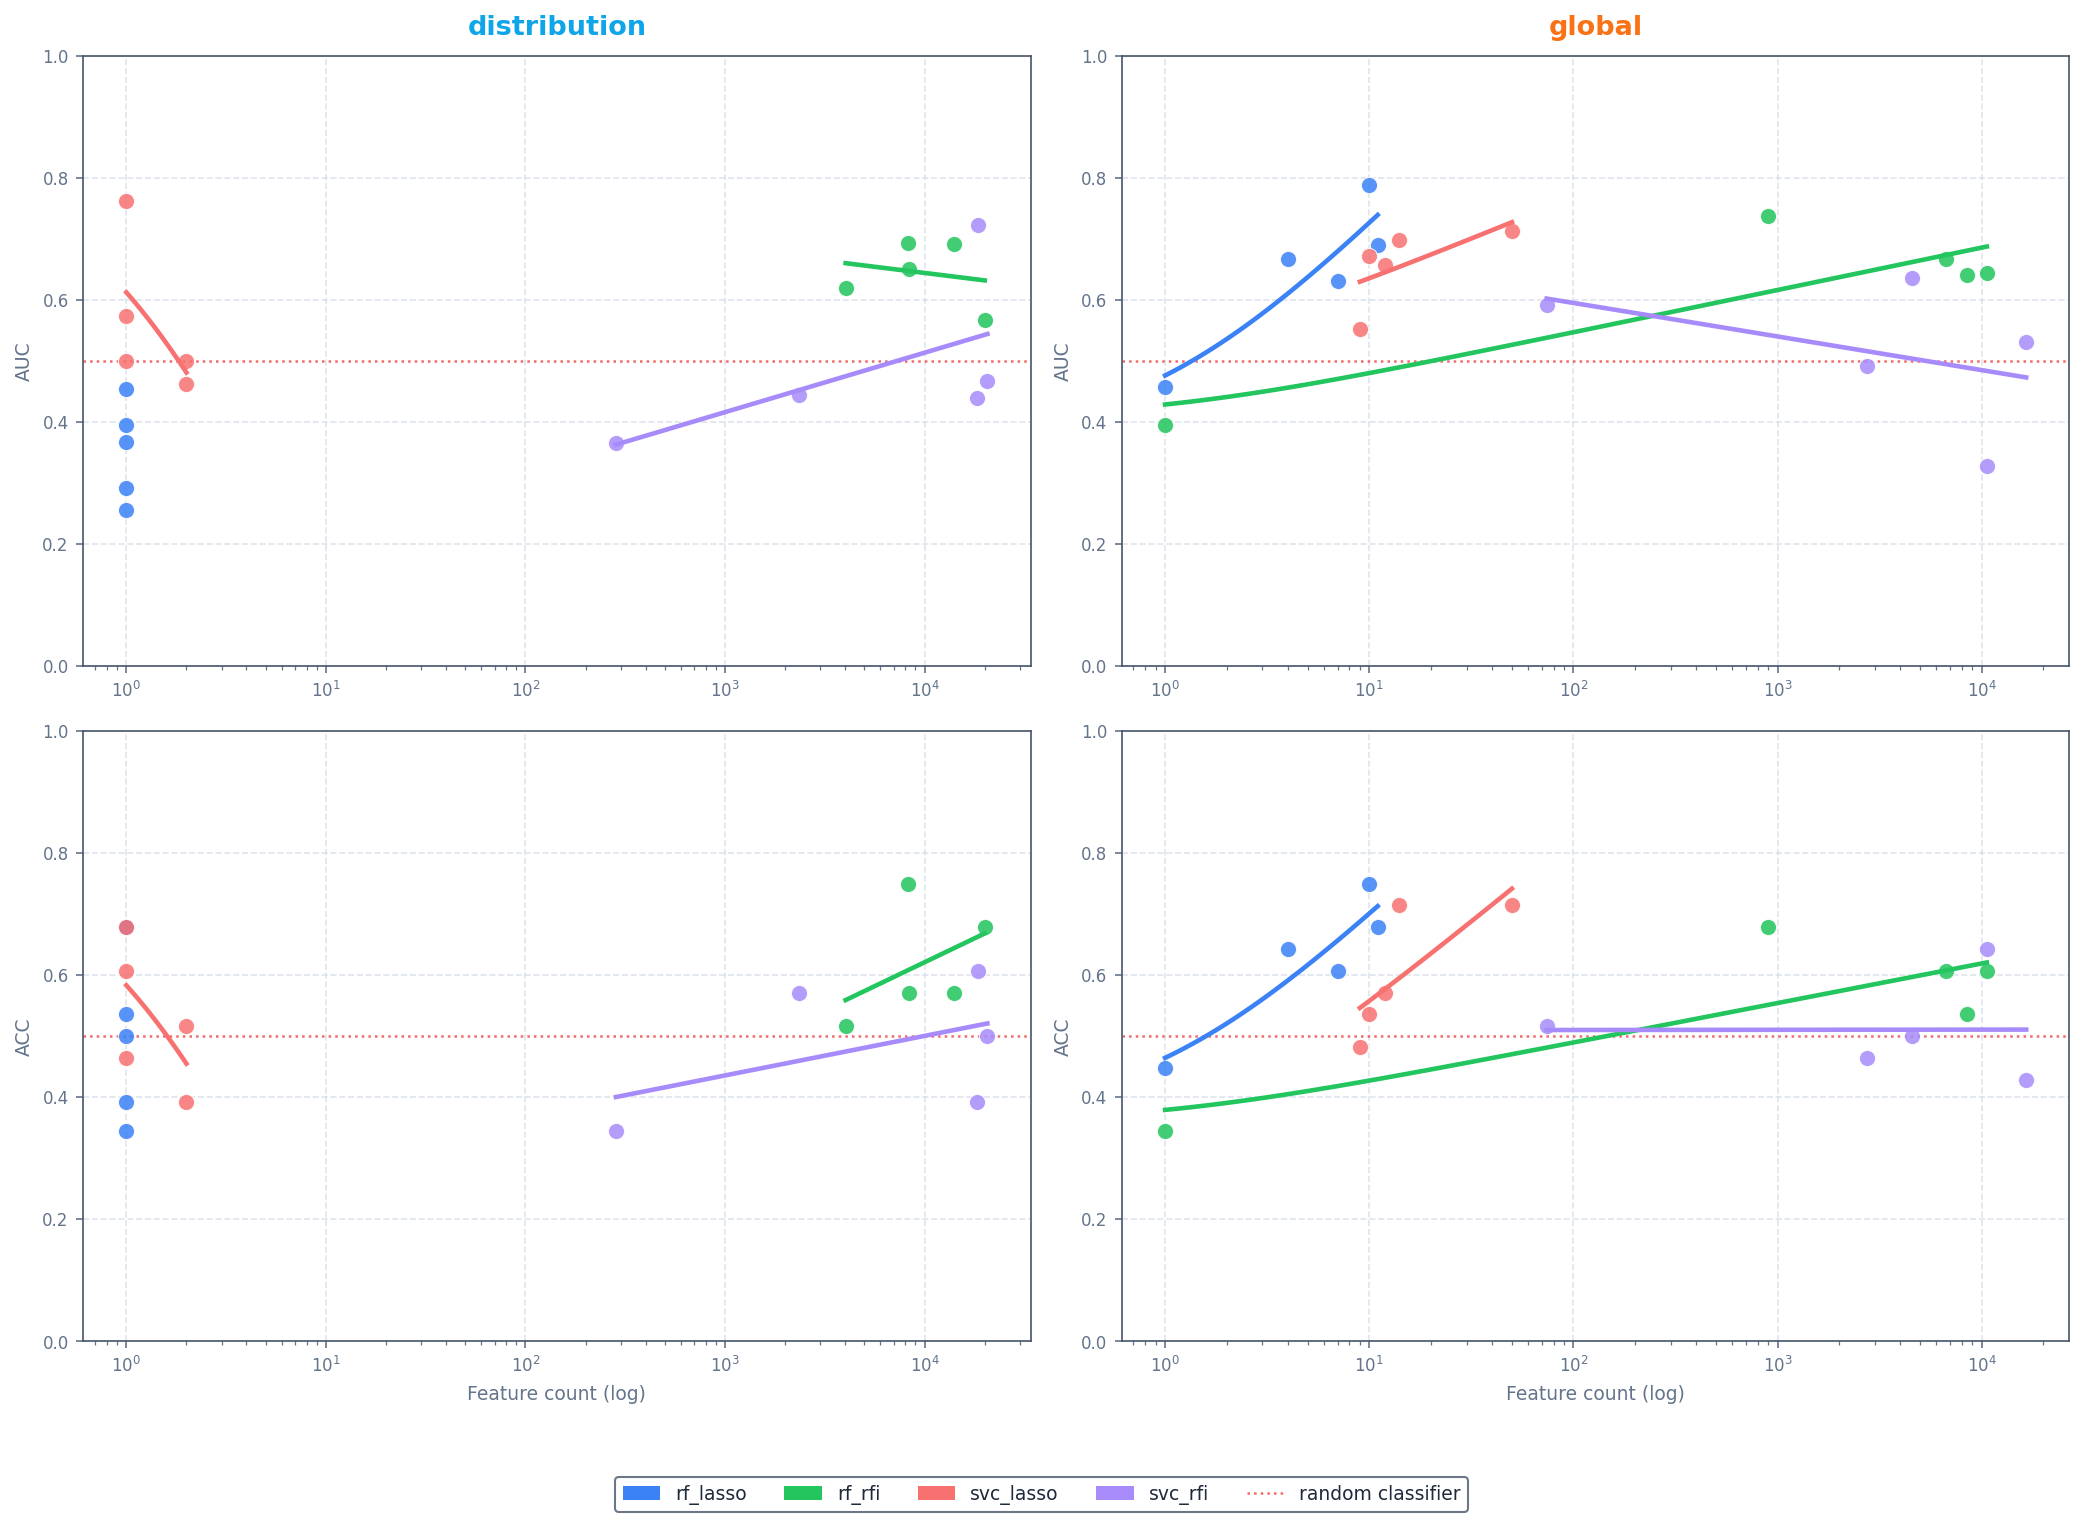
\includegraphics[width=1\textwidth]{img/spline_combined_dist_global.png}
\caption{Dependence of the AUC (top) and ACC (bottom) on the number of selected features for models trained on whole-thrombus feature sets. Each point represents results achieved for a single split. The number of selected features is shown on a logarithmic axis and ranges from 1 to more than $10^{3}$ out of 16528 features. Lines indicate linear regression trends fitted in log-space. RF: random forest classifier; SVC: support vector classifier; RFI: random forest importance-based selector; LASSO - least absolute shrinkage and selection operator selector.}\label{fig.spline_combined_dist_global}
\end{figure}

According to Fig.~\ref{fig.spline_combined_dist_global}, it is visible that models trained on the global-based dataset reached comparable or higher performance when selecting fewer than 100 out of 16528 features than those selecting more than 1000 features. Since models which used LASSO for feature selection achieve comparable AUC and ACC as the ones using RFI selector, the usage of these models is recommended as there is lower order of selected features, thus lower computational demand.

\begin{figure}[!htb]
\centering
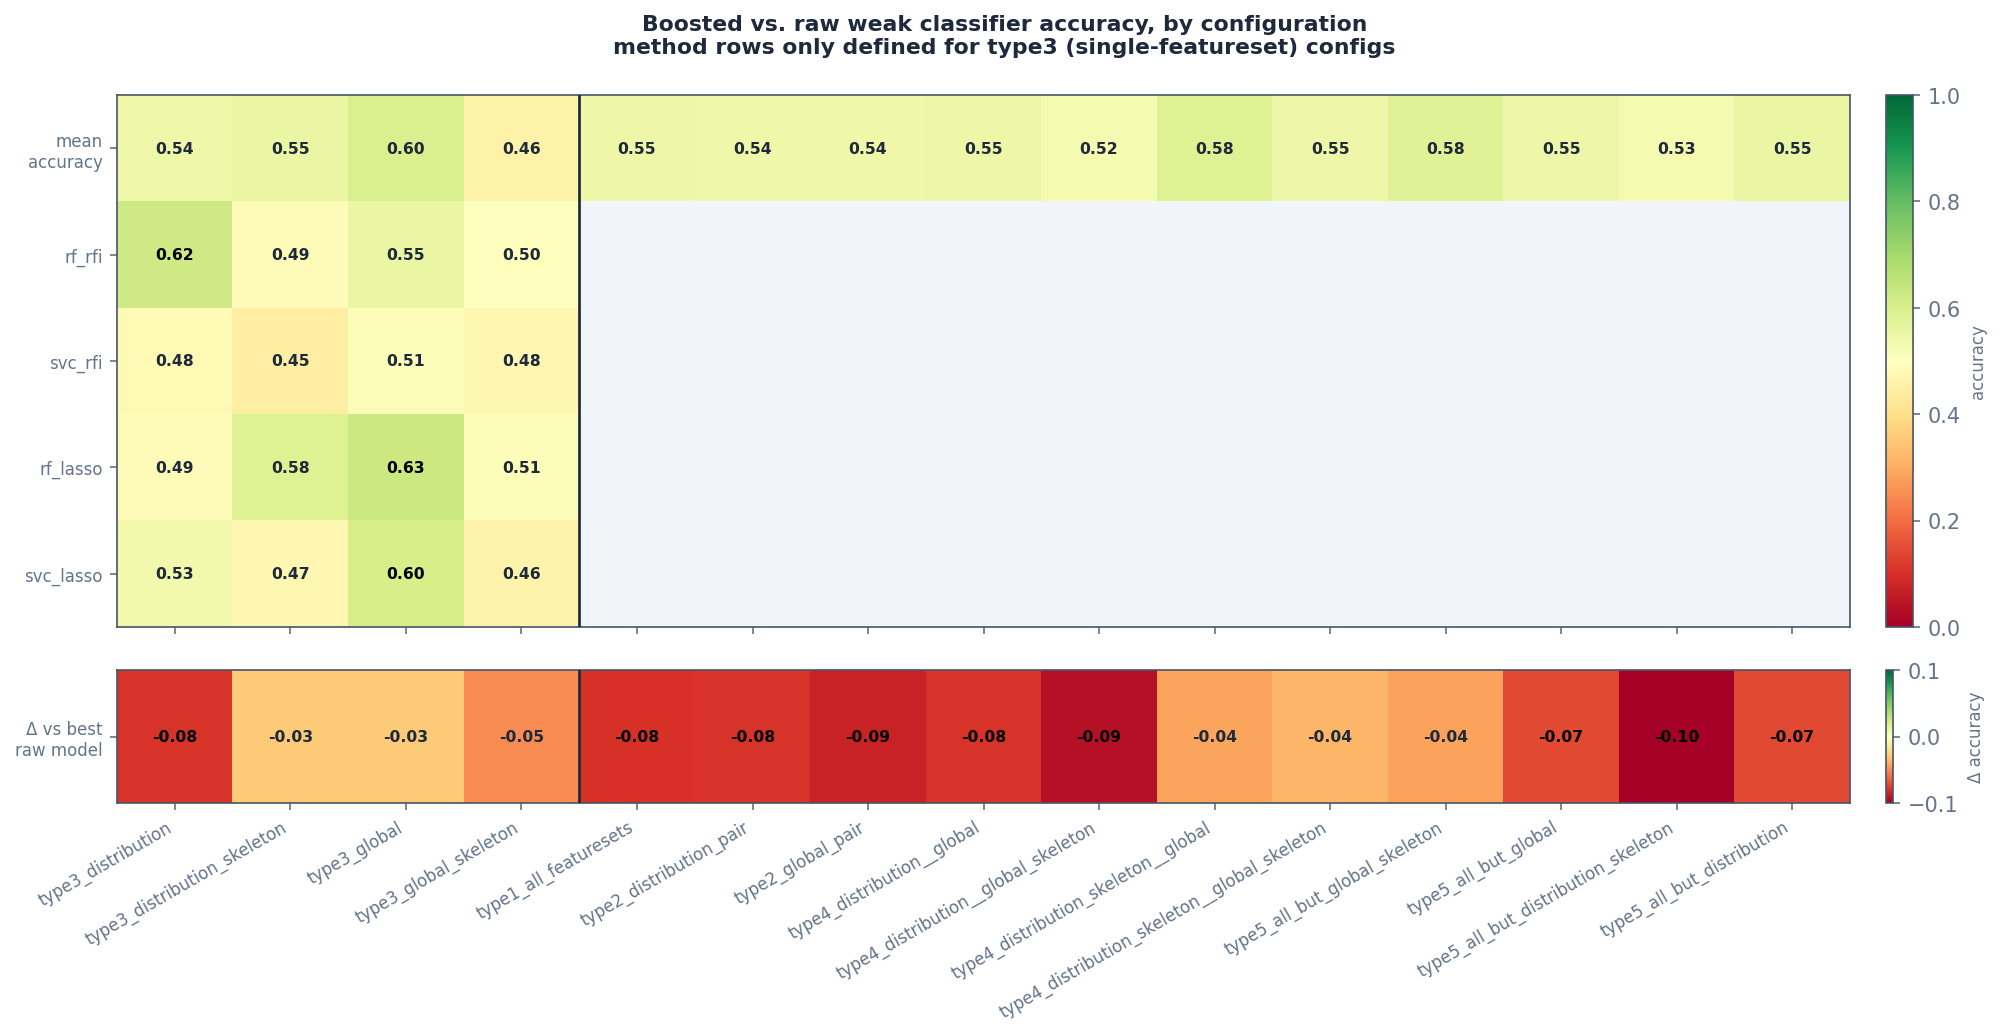
\includegraphics[width=1\textwidth]{img/boosted_vs_raw_accuracy_heatmap.png}
\caption{Accuracy of the boosted models and its difference from the individual models they combine. Columns represent the 15~evaluated ensemble configurations, ordered from configurations built on a single feature set (\emph{type3}, left of the divider) to configurations combining several feature sets (\emph{type1}, \emph{type2}, \emph{type4} and \emph{type5}). The top block shows the accuracy of the boosted model, both overall (\emph{mean accuracy}) and, for the configurations built on a single feature set, separately for each selector--classifier combination used as the weak learner. The shaded cells are not defined for the configurations combining several feature sets. The bottom strip shows the difference between the boosted model and the best individual model of the same configuration. RF: random forest classifier; SVC: support vector classifier; RFI: random forest importance-based selector; LASSO - least absolute shrinkage and selection operator selector.}
\label{fig.boosted_vs_raw_accuracy_heatmap}
\end{figure}

Registry - different population, older scanners

\section{Methods}\label{sec:methods}

\subsection{Study cohorts and outcome definition}

% 2.1 Study cohorts and outcome definition
% - Popis kohort (interná CV kohorta „NOIV" vs. externá „REGISTRY"), veľkosti, in/exclusion
For the purpose of this study, multicenter data from the MR CLEAN NO-IV trial dataset~\cite{Jansen2018}, including 539 patients with both NCCT and CTA scans and large vessel occlusion (LVO), were used to train, validate and test the prediction models. To increase the reliability of the study, the MR CLEAN Registry database~\cite{IvoGHJansen20180309} was used for feature reproducibility and model robustness testing.

% - eTICI≥2B ako binárny outcome, kto/ako labeloval

The patient inclusion and exclusion criteria for both datasets are described in \cite{Mojtahedi2024}. As reported in \cite{Nemcekova2025}, an additional exclusion step was required because of the feature extraction process, which reduced the NO-IV data set to 296 patients and the Registry database from 2597 to 1906 patients (16 missing TICI value, 575 missing thrombus segmentation, 100 spacing exceeding 1 mm). Thrombus segmentations were obtained using automated segmentation tool \cite{Mojtahedi2022312}. Since the NO-IV data set was used for model training, segmentations for this dataset were manually verified, and cases with inappropriate segmentation locations or multiple separated thrombus parts were excluded to ensure values from the valid image parts were used, reducing the training dataset to 141 patients.

The ratio of patients with successful reperfusion (SRP) to those with non-successful reperfusion (nSRP) was not adjusted, the final training dataset therefore consists of 82 patients with SRP and 59 patients with nSRP, preserving the same SRP to nSRP ratio as in the full dataset.

\subsection{Data preparation}

Since the database includes images from different scanners and therefore various resolutions, resampling the data to the same isotropic voxel size of~0.5~mm was crucial to ensure that the same amount of information is provided by each voxel. To prevent the impact of the marginal effects of the mask features and thus extract relevant feature values for whole thrombus, dilated segmentation mask was used for the feature extraction. A total of 1204 voxel-based features were extracted from both NCCT and CTA images using the PyRadiomics toolbox~\cite{VanGriethuysen20171031} with custom parameter settings described in the supplementary file \NOTETODO[PyradiomicsConfig.yaml]{PyradiomicsConfig.yaml -- not yet created}. Features with empty values were excluded before feature selection. This occurred due to the small size of the thrombus, which made the use of large filter masks not generalizable.

According to our preliminary study~\cite{Nemcekova2024}, determining the borders of the thrombus is challenging, and even experienced radiologists do not fully agree on the size of the segmented thrombi. Uncertain thrombus segmentation boundaries may introduce unwanted information from the clot neighborhood, mixing information from two different tissues and potentially introducing noise into extracted features. To investigate the influence of segmentation size, and specifically the impact of edge voxels on the prediction, only voxels located on the thrombus centerline, dilated by 3 voxels, were selected, defining the \textbf{core thrombus area}.

To explore the feature potential of information contribution, extraction of three feature sets at different levels of neighborhood influence was applied: voxel-based, distribution-based and global-based. \textbf{The voxel-based set} included 2064 radiomic feature values and NCCT and CTA values for each thrombus voxel. The \textbf{distribution-based set} was derived from the probability density across 10 bins of thrombus voxel-based feature histogram, which resulted in 20660 extracted features per patient. The \textbf{global-based set}, was based on global statistics computed from the feature values of the entire thrombus, including the voxel count, mean, standard deviation, minimum, maximum and the 25\%, 50\% and 75\% percentiles. Therefore, global based dataset included 16528 feature values per patient. As a result, six datasets (three feature set types and two region sizes) were used for the analysis.

To ensure that the division of the dataset into training and test sets did not affect the reproducibility of the predictions, the NOIV dataset was split into five non-overlapping training and testing folds. For the creation of the distribution-based feature set, histogram bin boundaries were defined from the training set. The definition of the splits in the context of the whole analysis pipeline is shown in the supplementary file \NOTETODO[XX]{Supplement/Thrombi_paper_FS_RF_SRP3.png}.

Each feature set underwent preprocessing, including z-score normalization based on the training set. The whole preprocessing pipeline is shown in Fig.\ref{fig.Thrombi_paper_FS_RF_SRP1}. 

\begin{figure}[!htb]
\centering
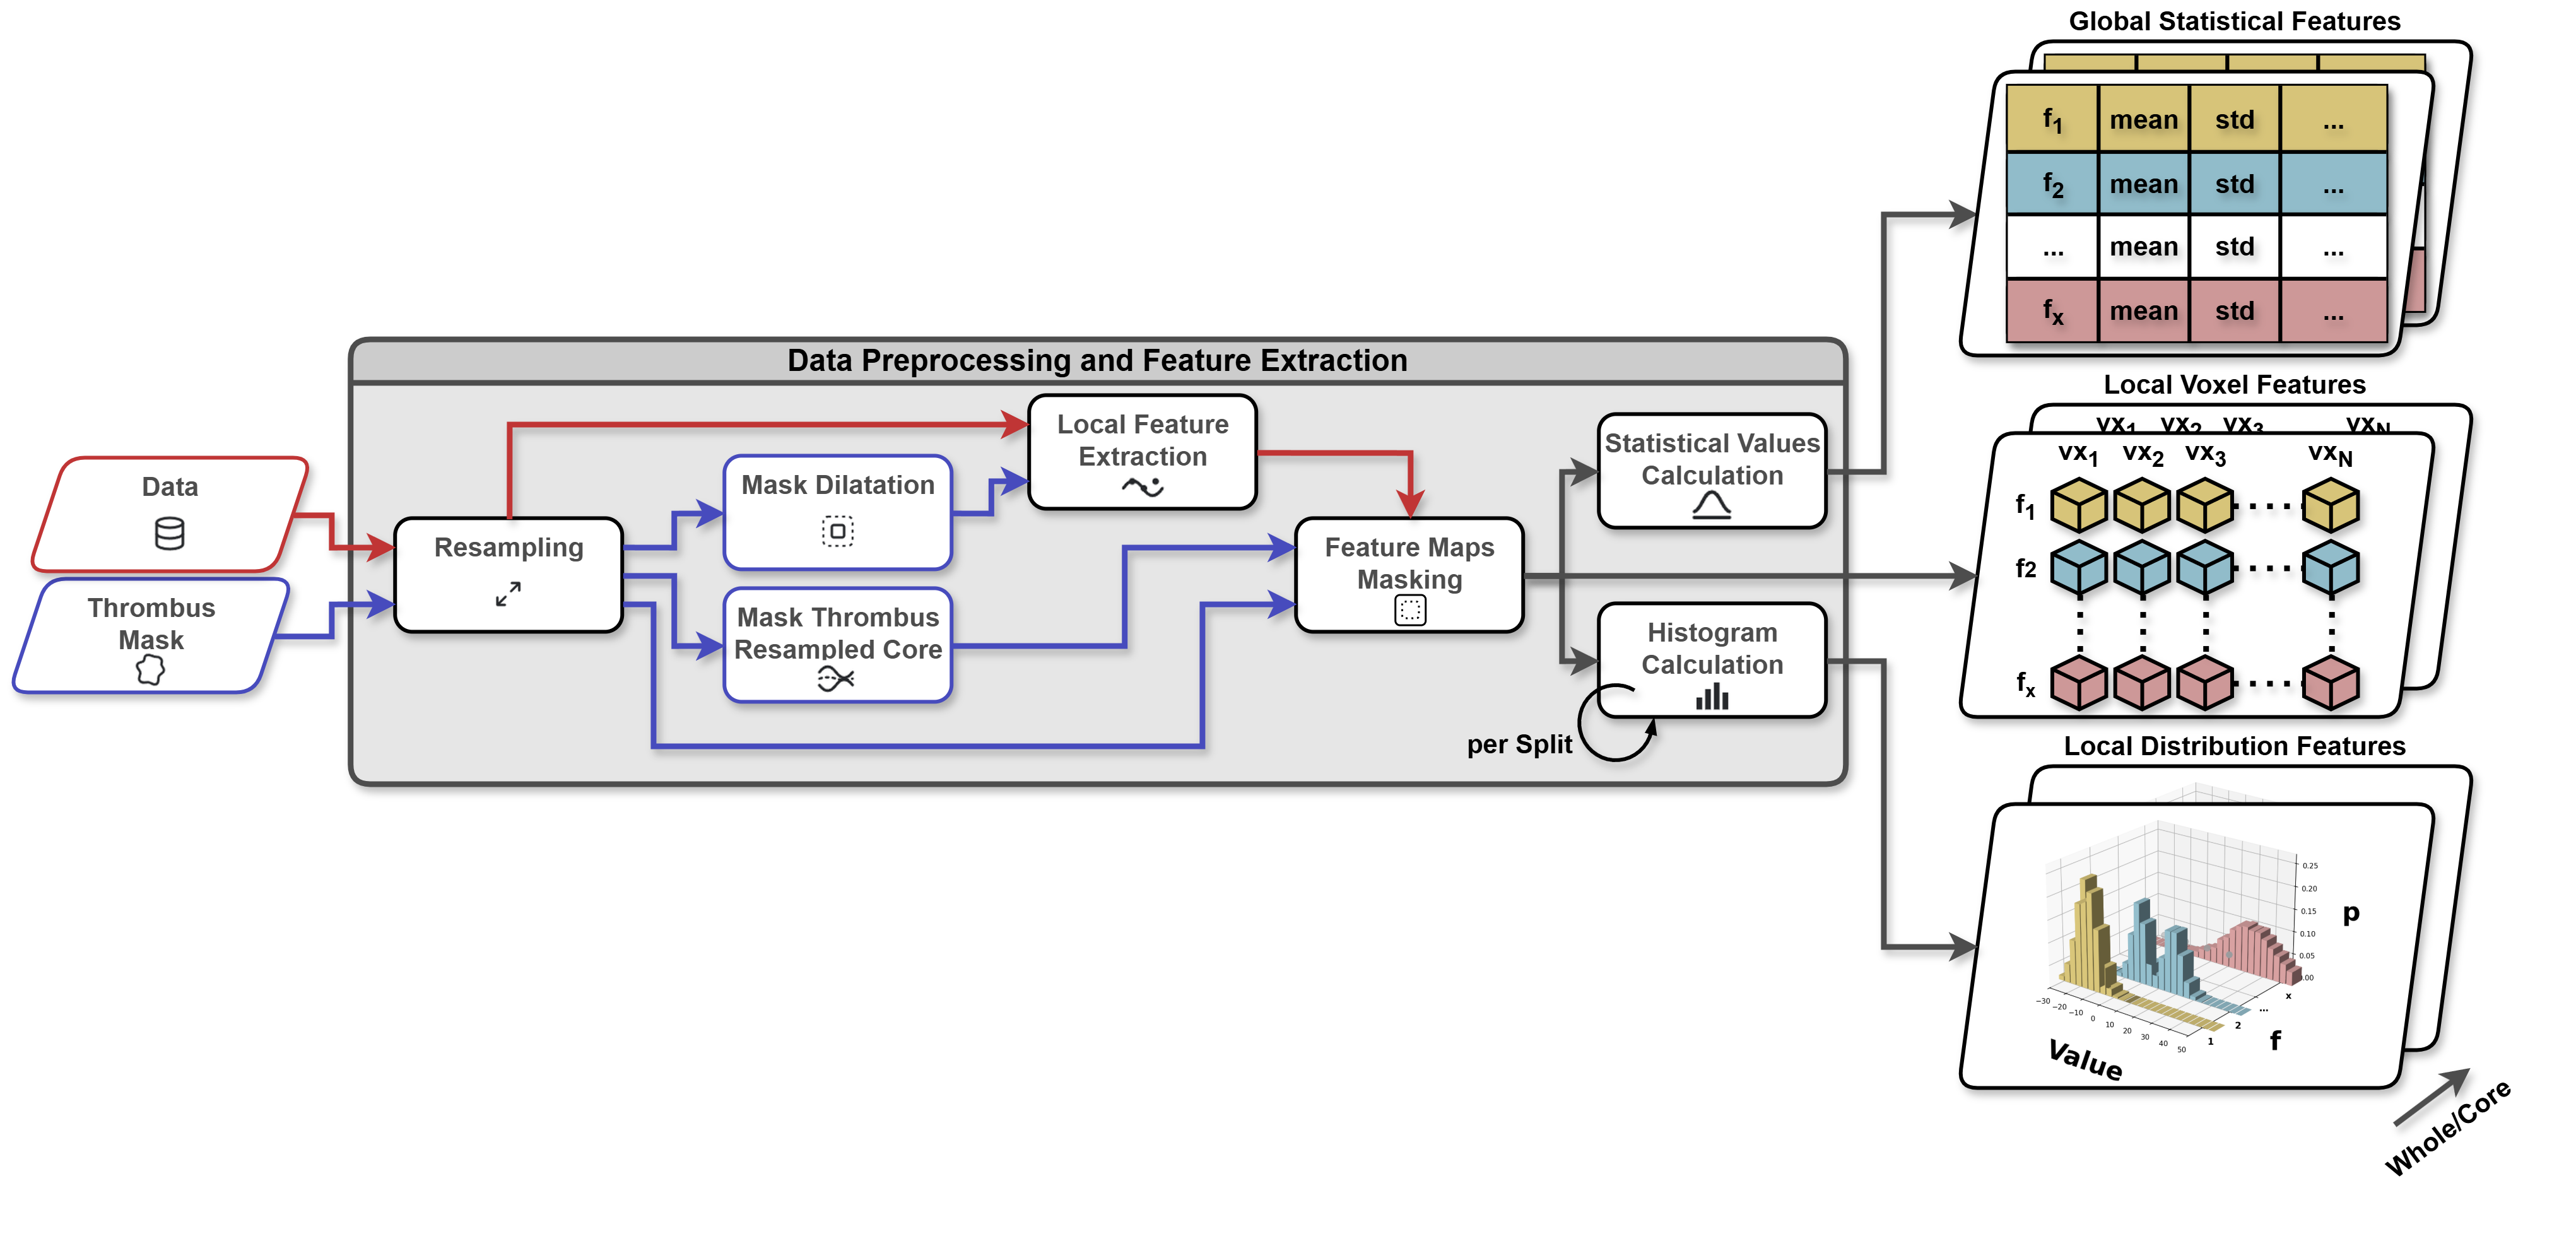
\includegraphics[width=1\textwidth]{img/Thrombi_paper_FS_RF_SRP1.png}
\caption{Data preprocessing pipeline. First, the data are resampled to the isotropic voxel size of~0.5~mm. Second, the thrombus mask dilation suppresses the impact of marginal effects during the feature extraction. Third, based on the selected area size, thrombus masking using the original thrombus mask (whole thrombus area) or core thrombus mask follows (core thrombus area). Based on the selection, the feature set creation finishes by this step (in case of voxel-based feature set), or continues by thrombus global statistics computation (global-based feature set) or thrombus feature histogram definition (distribution-based feature set). Thrombus histogram bin boundaries are defined by the training set. Data flow is represented by red lines, mask flow is represented by the blue line.}\label{fig.Thrombi_paper_FS_RF_SRP1}
\end{figure}

To define radiomic features that introduce an additional information for the diagnostic establishment and thus for the clinicians, the classification of the SRP/nSRP using the extracted features was performed. Since radiomics offers a large number of extracted features some of which may be redundant and may lead to model overfitting, feature selection was performed using two different methods. Feature selection using the Least Absolute Shrinkage and Selection Operator (LASSO) removed features with the coefficient value equal to zero. Second type of feature selection kept only predefined number of features with the highest XGBoost Random Forest Classifier Importance (RFI).

To ensure the selected classification method does not influence the outcome accuracy, a Support Vector Classifier (SVC) and XGBoost Random Forest Classifier (RF) were used.  All possible combinations of the selectors and classifiers were trained, resulting in four prediction method types (LASSO-SVC, LASSO-RF, RFI-SVC, and RFI-RF). This ensures that the definition of the most appropriate combination of the selector and classifier for this problem is established.

Parameter tuning was performed using Bayesian optimization with 20 trials. Feature selection and classifier training were treated as a single pipeline. Therefore, the Bayesian optimization was applied separately for each split, resulting in 120 trained models (3 dataset types x 2 area sizes x 5 folds x 4 methods), each with its own optimized parameter set and selected feature subset. The regularization parameter range for LASSO was defined according to Bickel et al., 2009 \cite{Bickel200981}. For the RFI selector, the number of features N was optimized, so that the top N features with sorted RFI values were selected. \NOTETODO[Table A1]{Detailed information about parameter setting and optimization needs an actual appendix table -- not yet created}. The final model for each combination of feature set, area of interest and method used was trained using the hyperparameters and selected features of the trial with highest accuracy during the optimization process. The whole process of model optimization and final model training is shown in Fig.\ref{fig.Thrombi_paper_FS_RF_SRP2}. 

\begin{figure}[!htb]
\centering
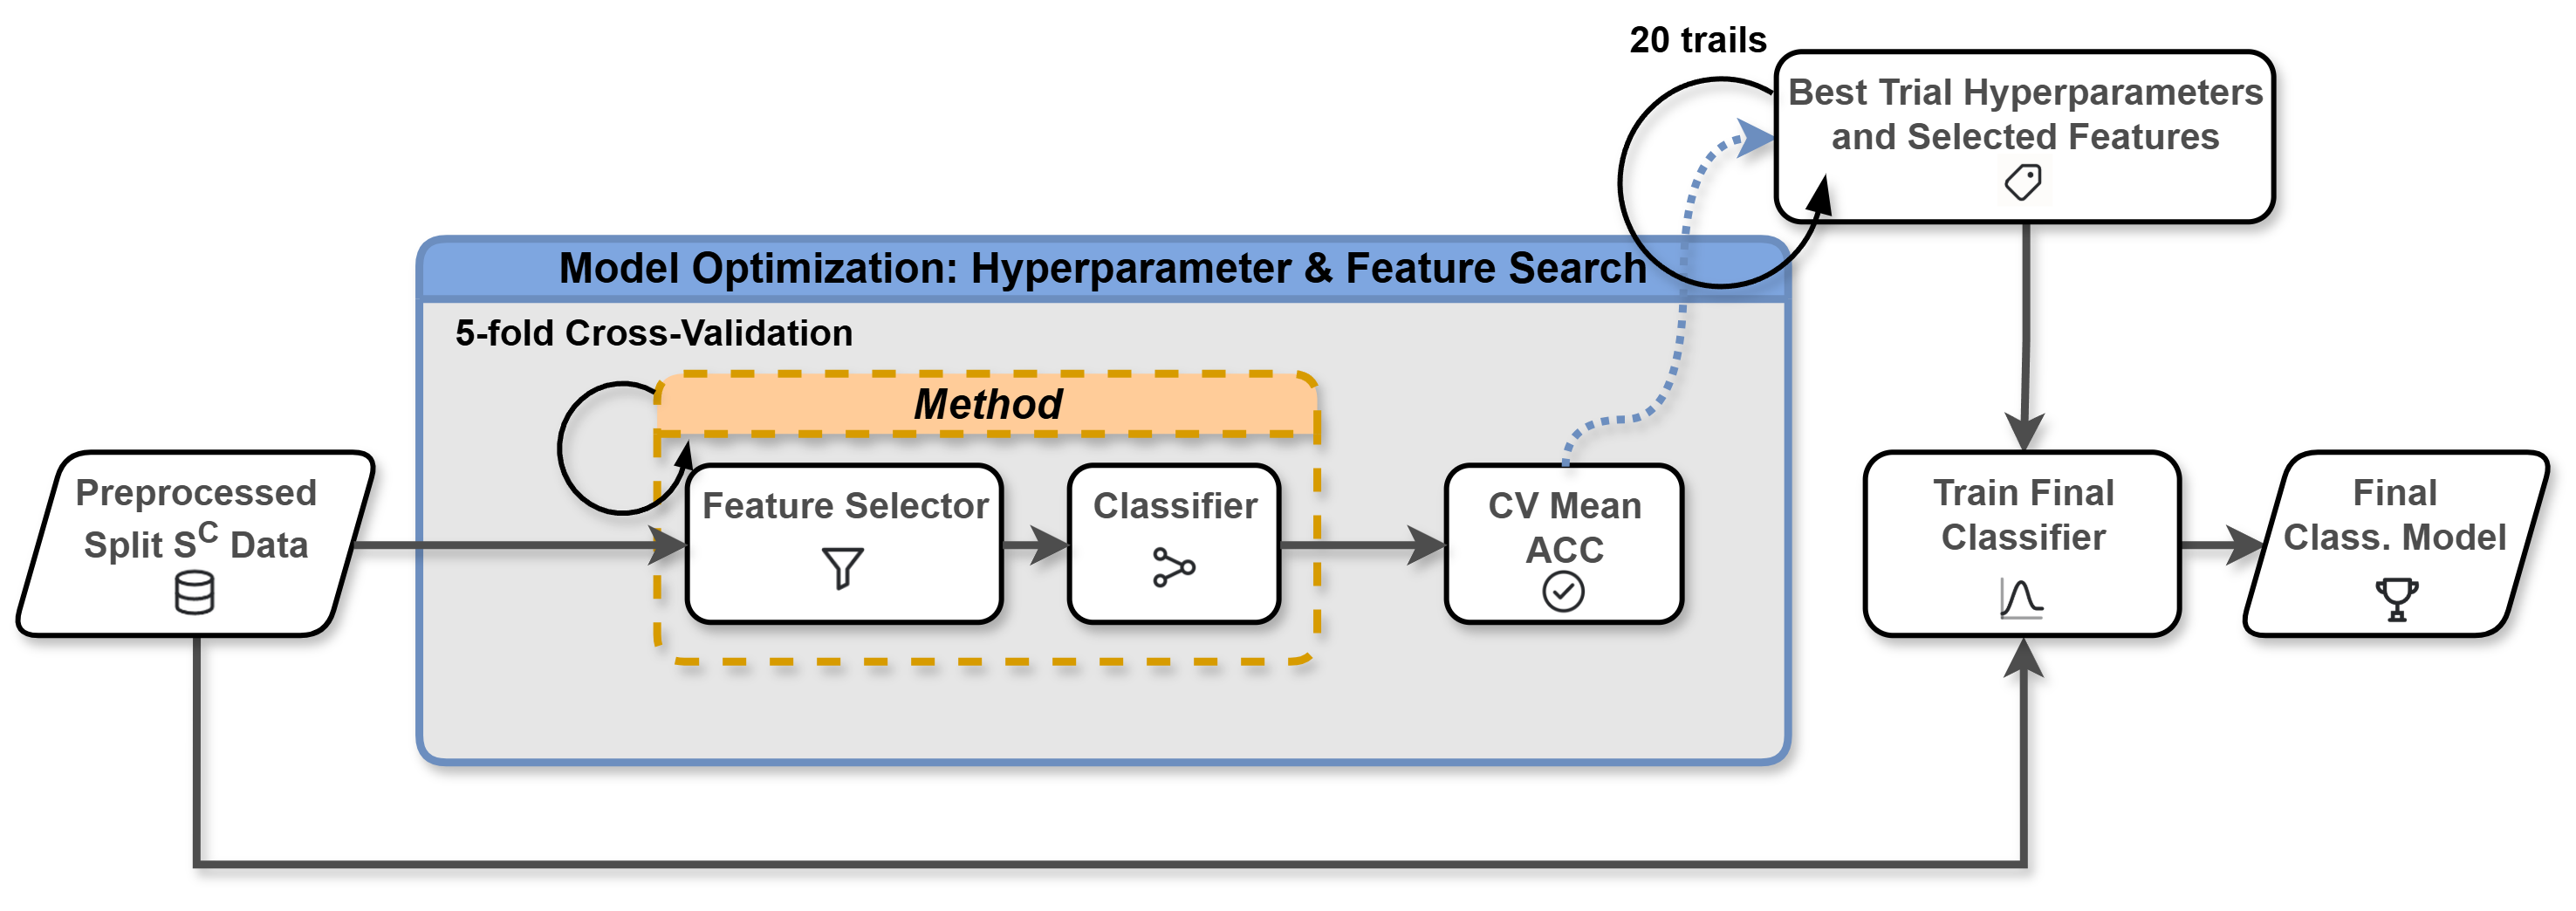
\includegraphics[width=1\textwidth]{img/Thrombi_paper_FS_RF_SRP2.png}
\caption{Model training and optimization pipeline. Hyperparameter optimization is performed using Bayesian optimization with 20 trials. After the process of optimization, the hyperparameter setting of the trial with the highest mean accuracy through 5 fold cross validation is used for the final model training. $S^C$: split's complement.}\label{fig.Thrombi_paper_FS_RF_SRP2}
\end{figure}

To support the green learning, only models for distribution and global based datasets were used for further model training and analysis, since all of the models using voxel based dataset predicted the same label. Thanks to the availability of REGISTRY independent testing dataset, optimization and training of models which used the whole NOIV database (all-fold models) for training was performed. This resulted in the creation of additional 16 all-fold models (2 dataset types - distribution and global based x 2 area sizes x 1 fold x 4 methods). To verify the possible predictive performance increase caused by the model combination, all combinations of models were provided to the boosting algorithm. Additional 16 boosted models were trained followed by the performance analysis.

All trained models are freely available and the framework is available on GitHub %\NOTETODO{PN}.

\subsection{Statistical analysis}
%\NOTETODO[dopsat statistickou analýzu]{domluvíme se ještě co všechno dodělat, a podle toho...}

To verify the influence of the feature set granularity and method used to establish the model performance, the predictivity of each model was determined separately. Using the permutation null-baseline analysis the investigation whether the trained model performance is higher than its stochastic variant. This consisted of shuffeling testing data labels before the ACC and AUC computation. The shuffeling followed by the metrics computation was performed 5000 times, to increase the These metrics were then used for the computation of the Cohen's Kappa as the metrics value of the random model instead of using a default value of 0.5.


The predictivity of all-fold models was determined using the independent testing database only.




\backmatter

\bmhead{Supplementary information}

Supplementary file \textit{B} contains the full per-combination AUC/ACC results for all methods, feature sets and regions of interest. The PyRadiomics extraction configuration is provided as \textit{PyradiomicsConfig.yaml}.

\bmhead{Acknowledgements}





\NOTETODO{Write the acknowledgements. The elsarticle draft's Acknowledgements section only contained a commented-out, now-stale \texttt{\textbackslash include\{tables\_tom/output/supplement\}} referencing a path that no longer exists in this repository -- dropped rather than carried forward.}

\section*{Declarations}

\begin{itemize}
\item Funding

\NOTETODO{State the funding source(s)/grant number(s). Not given in the elsarticle draft; the CRediT statement below credits Petra~Nemcekova with funding acquisition but no source is named.}

\item Conflict of interest/Competing interests

\NOTETODO{Supply an explicit competing-interests statement covering every author, or state that the authors declare no competing interests -- not stated in the elsarticle draft.}

\item Ethics approval and consent to participate

\NOTETODO{State the approving body and protocol/ethics reference number for the MR CLEAN NO-IV trial and MR CLEAN Registry data used here -- not stated in the elsarticle draft.}

\item Consent for publication

\NOTETODO{Confirm whether the manuscript contains any individually identifiable patient data/images requiring consent -- not stated in the elsarticle draft.}

\item Data availability

All trained models are freely available on and the framework is available on GitHub %\NOTETODO{PN}.

\NOTECHECK[freely available on and the framework]{This sentence is missing a word/repository name between "on" and "and" in the elsarticle draft -- carried forward as-is rather than guessed.}

\NOTETODO{State access conditions for the underlying MR CLEAN NO-IV/Registry patient data (typically restricted, not openly available) -- not stated in the elsarticle draft.}

\item Materials availability

\NOTETODO{Not stated in the elsarticle draft.}

\item Code availability

The training/evaluation framework is available on GitHub (see Data availability above).

\item Author contribution

Petra~Nemcekova: Conceptualization, Data curation, Formal analysis, Funding acquisition, Investigation, Methodology, Project administration, Software, Validation, Visualization, Writing -- original draft, Writing -- review \& editing. Jiri~Chmelik: Conceptualization, Project administration, Supervision, Visualization, Writing -- original draft, Writing -- review \& editing. Tomas~Vicar: Conceptualization, Supervision, Writing -- original draft, Writing -- review \& editing. Mahsa~Mojtahedi: Data curation, Writing -- review \& editing. Agnetha~E~Bruggeman, Henk~van~Voorst, Elena~Ponomareva, Manon~Kappelhof, Aad~van~der~Lugt, Jan~W~Hoving, Bruna~G~Dutra, Diederik~Dippel, Fabiano~Cavalcante, Lonneke~Yo, Jonathan~Coutinho, Josje~Brouwer, Kilian~Treurniet, Manon~L~Tolhuisen, Natalie~LeCouffe, Nerea~Arrarte~Terreros, Praneeta~R~Konduri, Wim~van~Zwam, Yvo~Roos, Charles~B~L~M~Majoie, Bart~J~Emmer: Data curation. Henk~A.~Marquering: Resources, Supervision, Writing -- review \& editing. Roman~Jakubicek: Conceptualization, Project administration, Supervision, Writing -- original draft, Writing -- review \& editing.

\end{itemize}

\begin{appendices}

\section{Parameter setting and optimization}\label{secA1}

\NOTEWARN[Table A1 is referenced but does not exist]{The Methods section refers to ``Table A1'' (\texttt{Detailed information about parameter setting and optimization}) but no such table was ever created in the elsarticle draft -- only the in-text reference survived. Needs an actual table here, labelled \texttt{tab:placeholder-A1}, before submission.}



Conclusion 1 - global and distribution based features are helpful, voxel based features do not make sense for prediction
Conclusion 2 - even though in distribution and global based features are statistically singnificant difference between random model and trained model, performance of these models is poor
Conclusion 3 - models are not generalized and do not work on different datasets



\end{appendices}

\bibliography{BibFile}

\end{document}
